\documentclass[answers]{exam}
\usepackage[utf8]{inputenc}
\usepackage{graphics}
\usepackage{amssymb}
\usepackage[export]{adjustbox}
\usepackage{hyperref}
\hypersetup{
    colorlinks=true,
    linkcolor=blue,
    filecolor=magenta,      
    urlcolor=blue,
}
\urlstyle{same}
\graphicspath{ {./images/} }
\everymath{\displaystyle}

\title{CS 451: Computational Intelligence \\ \Large Final Project}
\author{Proposal}
\date{\today}

\begin{document}
\maketitle
\paragraph{} \centering
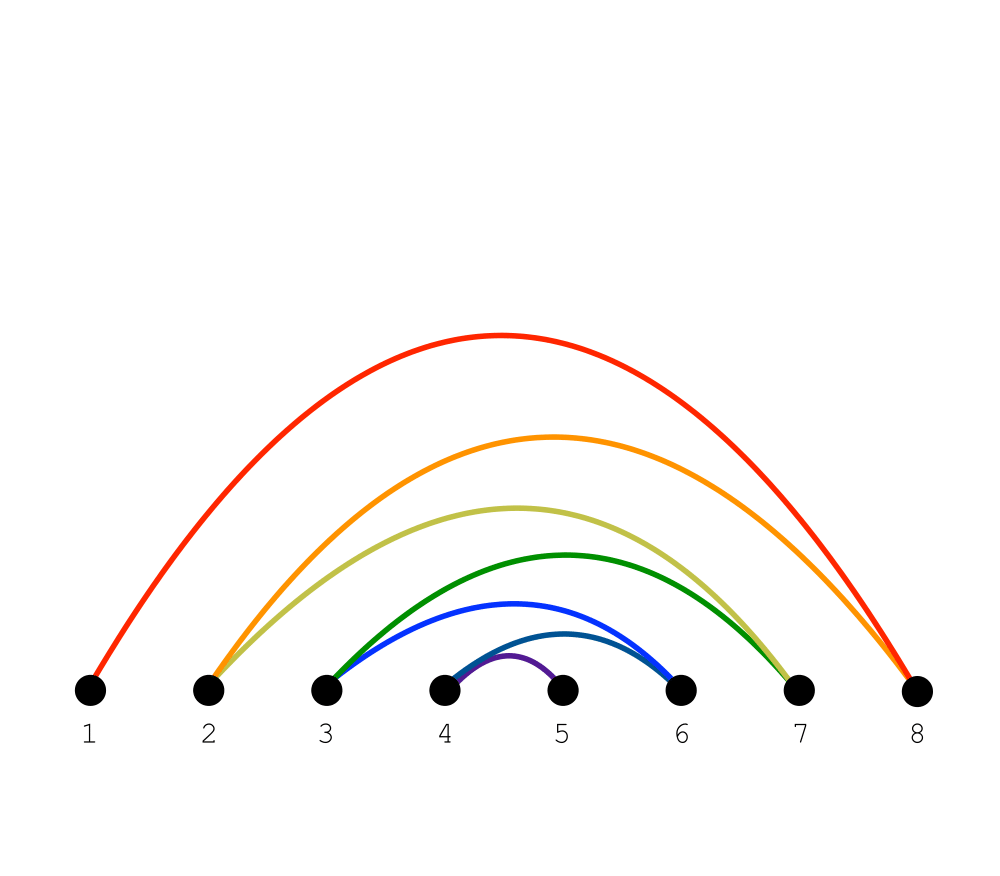
\includegraphics[scale=0.4]{cover.png}
\paragraph{} \flushleft


\newpage
\tableofcontents

\newpage
\section{Introduction \& Logistics}
\paragraph{}
\paragraph{Topic:} Graph Bandwidth Problem
\paragraph{Section:} L1 - Dr. Saleha Raza
\paragraph{Group Members:}
\paragraph{}
*All names appear in alphabetical order; any other apparent pattern is purely coincidental.
\begin{enumerate}
    \item Maaz Saeed - ms05050
    \item Maham Shoaib Patel - mp04911
    \item Muhammad Usaid Rehman - mr04302
\end{enumerate}

\section{Graph Bandwith Problem}


\subsection{Problem Definition}
\subsection{Runtime Complexity \& Approximation Algorithms}

\section{Potential Strategy}

\subsection{Justification}

\section{Software \& Applications}
Python - NetworkX, and NumPy

\end{document}